\documentclass{article}

% ------ PACKAGES ------ %

% \usepackage{times}
% \usepackage{palatino}
% \usepackage{mathptmx}
\usepackage{charter}
\usepackage{geometry}
\usepackage{amsmath}
\usepackage{amssymb}
\usepackage{float}
\usepackage{subcaption}
\usepackage{enumitem}
\usepackage{titlesec}
\usepackage{hyperref}
\usepackage{xcolor}
\usepackage{fancyvrb}
\usepackage{tikz}
\usepackage{pgfplots}

\usetikzlibrary{positioning}

% ---------------------- %

% ------ GENERALS ------ %

\geometry{margin=1in}

\setlist[itemize]{label=\scriptsize\textbullet}
\setlist[itemize]{noitemsep, topsep=1pt}
\setlist[enumerate]{noitemsep, topsep=1pt}

% \setcounter{tocdepth}{3}
% \setcounter{secnumdepth}{3}

\titleformat{\chapter}[hang]
    {\normalfont\huge\bfseries}{\thechapter}{1em}{}

% ---------------------- %

% ------- COLORS ------- %

\definecolor{ccode}{RGB}{0, 0, 192}

\DefineVerbatimEnvironment{verbatim}{Verbatim}
    {fontfamily=courier, fontsize=\small, formatcom=\color{ccode}}

\RenewDocumentCommand{\verb}{v}
    {\begingroup\color{ccode}\fontfamily{pcr}\selectfont#1\endgroup}

\hypersetup{
    colorlinks=true,
    linkcolor=black,
    urlcolor=blue,
    citecolor=blue,
    pdfborder={0 0 0}
}

% ---------------------- %

% ------ COMMANDS ------ %

\newcommand{\newpar}[0]{\vspace{2mm}\noindent}
\newcommand{\htitle}[1]{\newpar\textbf{#1 -}}
\newcommand{\hyperlabel}[1]{\hypertarget{#1}\phantomsection\label{#1}}
\newcommand{\hyperitem}[2]{\item \hyperlink{#1}{#2}\leaders\hbox to 0.8em{\hss.\hss}\hfill\hbox to 1.8em{\hss\pageref{#1}}}
\newcommand{\stdtilde}[0]{\raise.17ex\hbox{$\scriptstyle\sim$}}
\newcommand{\xor}[0]{\char`\^}
\newcommand{\saveformula}[2]{\newbox{#1}\savebox{#1}{#2}}
\newcommand{\useformula}[1]{\usebox{#1}}
\newcommand{\ul}[1]{\underline{#1}}
\newcommand{\ol}[1]{\overline{#1}}

\newcommand{\frontpage}[3]{
    \title{
        \fontsize{30}{36}\selectfont #1
        \\[2.5cm] \Large #2
    }
    \author{#3}
    \date{\today}
    \maketitle
    \newpage
    \tableofcontents
    \newpage
}

% ---------------------- %

\begin{document}

% -------- HEAD -------- %

\title{\Huge Foundations of Operations Research}
\author{Francesco Ostidich}
\date{\today}
\maketitle
\vspace{12mm}
\tableofcontents
\newpage

% ---------------------- %

\section{Introduction}

\subsection{Decision making problems}

Decision making problems can be arranged in various categories:

\begin{itemize}
    \item \textbf{matematical programming} has a single decision maker and a single objective;
    \item \textbf{multi-objective programming} has instead several objectives;
    \item \textbf{stochastic programming} corresponds to problems where there is a uncertainty level;
    \item \textbf{game theory} fits well when there are multiple decision makers.
\end{itemize}

\subsubsection{Mathematical programming}

Mathematical programming opts to minimize a decision variable $x \in \mathbb{R}^n$ inside a feasible region $X \subseteq \mathbb{R}^n$
via a objective function $f: x \rightarrow \mathbb{R}$.

MP is categorized in three special cases.

$$X_0 = \Biggl\{ x \in \mathbb{R}^n : g_i(x) \lesseqgtr 0 , i=1, 2, 3, \dots, m \Biggr\}$$

\begin{itemize}
    \item \textbf{Linear programming} (LP): $X = X_0$, with $f$ and $g$ linear
    \item \textbf{Integer linear programming} (ILP): $X = X_0 \cap \mathbb{Z}^n$, with $f$ and $g$ linear
    \item \textbf{Non linear programming} (NLP): $X = X_0$, with $f$ and $g$ non linear
\end{itemize}


\section{Graph and network optimization}

\subsection{Graph reachability problem}

Given a graph $G = (N,A)$ and a node $s$, find all nodes that are reachable from $s$.

Efficient algorithms use queues to keep track of previously expanded nodes; different objectives are pursued based on the queue type, each with its complexities.

\subsection{Minimum spanning tree}

Given a graph $G = (N,E)$, with each edge having a cost $c_e \in \mathbb{R}$, find a spanning tree $G_T = (N,T)$ with minimum total cost.
Being $X$ the set of all the spanning trees of $G$, the objective is to find

$$ \min_{T \in X} \sum_{e \in T} c_e $$

that may not be a easy task being the number of spanning trees $2^{n-2}$, with $n$ the number of nodes of the graph.

\subsubsection{Kruskal method}

Firstly, the arcs list is ordered from the least costly to the most costly.
Then, one arc after the other, they are popped and added to the graph.
If adding an arc would create a cycle, it is skipped.
In the end, what does remain is the minimum spanning tree.

\subsubsection{Prim's algorithm}

The spanning tree is built iteratively, starting from an initial tree $(S,T)$, where $S={u}$ and $T=\emptyset$.

At each iteration, the edge with the lower cost (among the unchosen edges of the cut $S$) is added to $T$, and the node it connects to $S$.

The complexity of the algorithm is $O(nm)$, being $n$ the number of nodes and $m$ the number of edges.

This algorithm is exact, since it always provides an optimal solution.
It is also greedy, since it look for the local minima iteratively, without reconsidering previous choices.

\newpar
A variance of the Prim's algorithm with complexity $O(n^2)$ can be achieved by associating each node with another.
Each node $i$ is assigned with another node $j$, that is either the predecessor (if $i \in S$), or the one in the spanning tree with which it has minimum cost ($\mathrm{argmin}_{i,j} c_{ij}$).

This way, with each iteration, it is faster to choose the node with minimum cost that connects to the newly expanded node.

\subsection{Dijkstra's algorithm}

Dijkstra's algorithm can be used to find the shortest path from a node to all other nodes of the graph.

Each node is assigned a label storing the cost of the current shortest path found, along with the predecessor in that path.
At each iteration nodes in the frontier are expanded, and if the new path for the neighboring is shorter than their previous, the labels of the are updated.

If all $m$ arcs are scanned the complexity is $O(mn)$, but if labels are appropriately updated complexity becomes $O(n^2)$.
Dijkstra's algorithm is exact, meaning it always provides an optimal solution.
It does not work with negative cost arcs.

The tree made from the set of short paths for a node $s$ is called the arborescence rooted at $s$.

\subsection{Floyd-Warshall algorithm}

This algorithm can be used when the graph contains paths with negative costs.

The graph is to be described via a matrix $D$, in which each cell is the cost between the row and column nodes.
Along with $D$, define a matrix $P$ which, in the end, $p_{ij}$ is the predecessor of $j$ in the shortest path from $i$ to $j$.

$$
D=
\begin{bmatrix}
    0 & 2 & \infty & 1 \\
    \infty & 0 & 3 & 3 \\
    \infty & 0 & 2 & \infty \\
    \infty & -5 & 5 & \infty
\end{bmatrix}
\hspace{2.5cm}
P=
\begin{bmatrix}
    1 & 1 & 1 & 1 \\
    2 & 2 & 2 & 2 \\
    3 & 3 & 3 & 3 \\
    4 & 4 & 4 & 4
\end{bmatrix}
$$

Then, for each $u = 1, \dots, n$, if $d_{iu} + d_{uj} < d_{ij}$, then $d_{ij} = d_{iu} + d_{uj}$.
If the path cost is updated, then the corresponding element of the $P$ matrix is updated to $u$.

The Floyd-Warshall algorithm is exact, with complexity $O(n^3)$, being $n$ the number of nodes.

\subsection{Topological ordering method}

A DAG (directed acyclic graph) can be rearranged so that, for every path $(i, j)$, an order $i < j$ is defined.

Each "layer" of the topological ordered graph is found iteratively, starting from a node which has no incoming edge.
With each iteration, fill the following layer with the nodes directly reachable from the current.

Complexity is $O(n+m)$, since each node and each arc is considered once.

\subsection{Dynamic programming}

Dynamic programming is a technique for which an optimal solution is found by resolving a set of recursive equations.
It can be applied to decision problems that satisfy the optimality principle, stating that if a path from node $1$ to $j$ is the shortest, than the path from $1$ to $i$, where $i$ is the predecessor of $j$ in the path, is also optimal.

\subsubsection{Shorter path in DAGs}

Let $L_n$ be the cost of the path between node $1$ and $n$.
If the objective is to find the minimum-cost path from $1$ to $i$, then the problem becomes to minimize the value of $$L_{j} + c_{ji}$$ where $j$ is the predecessor of $i$ and $c_{ji}$ is the cost between $j$ and $i$.

For example, the set of recursive equations that describe the problem may be

\begin{align*}
    \textrm{pred}_i = 1 &, \quad L_1 = 0 \\
    \textrm{pred}_i = 1 &, \quad L_2 = L_1 + c_{12} = 4 \\
    \textrm{pred}_i = 1 &, \quad L_3 = L_1 + c_{13} = 2 \\
    \textrm{pred}_i = 3 &, \quad L_4 = \min_{i=1,2,3}\{L_i + c_{i4}\} = \min\{0+5, 4+2, 2+1\} = 3
\end{align*}

where, with each iteration over the formulae, the cost and predecessor of each node is updated until the formula for the final node has no dependencies left over.

\subsection{Project planning}

A project is a set of activities each with its duration.

Activities may have a precedence constraint, for example $A_i \propto A_j$.
In those cases, the starting node of $A_j$ must appear after the ending node of $A_i$.

Between activity arches, dummy arcs can be added to symbolize dependencies.
Artificial nodes and arcs may also be added in order to obtain a single initial and final node.

\begin{figure}[H]
    \centering
    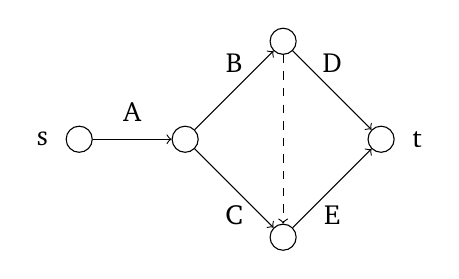
\begin{tikzpicture}[state/.style={circle, draw, minimum width=1mm}]
        \node[state] (A) {};
        \node[left = 0.1cm of A] {s};
        \node[state] (B) [right = of A] {};
        \node[state] (C) [above right = of B] {};
        \node[state] (D) [below right = of B] {};
        \node[state] (E) [below right = of C] {};
        \node[right = 0.1cm of E] {t};
        \path (A) edge [->] node[above = 0.1cm] {A} (B);
        \path (B) edge [->] node[above = 0.1cm] {B} (C);
        \path (B) edge [->] node[below = 0.1cm] {C} (D);
        \path (C) edge [->, dashed] (D);
        \path (C) edge [->] node[above = 0.1cm] {D} (E);
        \path (D) edge [->] node[below = 0.1cm] {E} (E);
    \end{tikzpicture}
\end{figure}

\subsubsection{Critical path method}

The CPM is used to determine a schedule, that is the set of activities that minimizes the total project duration, and the slack of each activity, that is maximum time an activity can be delayed.

After constructing the graph of activities in topological order, find

\begin{enumerate}
    \item the earliest time $T_{min}$ for each node with increasing indices,
    \item the latest time $T_{max}$ for each node with decreasing indices,
    \item the slack for each activity $\sigma_{ij} = T_{max, j} - T_{min, i} - d_{ij}$.
\end{enumerate}

A critical path is one that has slack equal to zero.

\subsection{Network flow}

A network is a directed and connected graph, that contains both a source (a node with only outgoing arcs) and a sink (a node with only ingoing arcs).

Each arc of the graph can be assigned with a value in order to produce a feasible flow.
This values must satisfy both the capacity constraint, meaning that the value must be less than the arc original cost, and the flow balance constraint, stating that the sum of the ingoing arc values for a node must be equal to the outgoings.

The value of flow is the sum of outgoing values from the source node.
An arc is saturated if the assigned value is the same as the cost, or else it is empty if it is zero.

A cut of the graph has a capacity equal to the sum of the outgoing arcs costs, and given a feasible flow, this has a value through the cut equal to the difference between ingoing and outgoing arc values.

Given a feasible flow, each cut $S$ of the graph has a value $\phi$ of the flow that is equal to the one of the source node: $\phi(S) = \phi(\{s\})$.
Furthermore, the value of the flow is always less than the capacity of the cut: $\phi(S) \le k(S)$.
If $\phi(S) = k(S)$ then the the feasible flow $\underline{x}$ is of maximum value and the cut $\delta(S)$ is of minimum capacity.
From here, two main problem arise: the primal problem consists of finding a feasible flow of maximum value; the dual problem consists of finding a cut of minimum capacity.

\subsubsection{Ford-Fulkerson algorithm}

The Ford-Fulkerson algorithm is a method for computing the maximum flow in a flow network. It is based on the idea of finding augmenting paths and increasing the flow along these paths until no more augmenting paths can be found.

Firstly, initialize the graph by setting all edge flows to zero.
Then, with each iteration, find a path from the source to the sink where the available capacity is greater than the current flow and increase the flow along this path by the smallest available capacity on the path (the bottleneck).
After augmenting the flow, update the residual capacities of the edges.
This process is to be repeated until no more augmenting path can be found.

This algorithm is non-greedy and exact.
The complexity is $O(m^2k_{max})$, where $m$ is the number of arcs and $k_{max}$ is the biggest capacity among all the arcs.
The algorithm can be inefficient in some cases, but when dealing with integer capacities it is possible to reduce complexity to be polynomial using other algorithm implementations.

\newpar
The theorem of strong duality derived from this algorithm tells that the value of a feasible flow of maximum value equals to the capacity of a cut of minimum capacity.


\section{Linear programming}

\subsection{Graphic example}

\begin{align*}
    f(x_1, x_2) & = 0.04 x_1 + 0.06 x_2 \\
    x_1 + x_2 & \le 10000 \\
    x_1 & \le 7500 \\
    x_2 & \le 5000 \\
    x_1, x_2 & \ge 0
\end{align*}

Let $f(x_1, x_2)$ be the function to maximize.
The feasible region, in which the variables satisfy the constraints, can be plot graphically.

\begin{figure}[H]
    \centering
    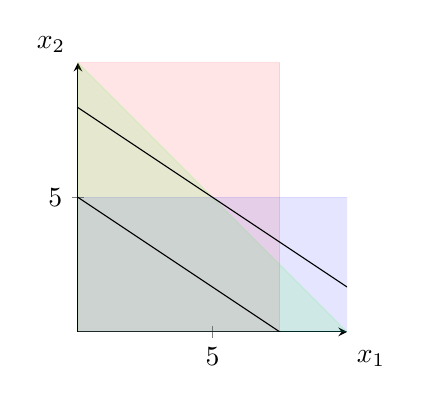
\begin{tikzpicture}
        \begin{axis}[
            axis lines=middle,
            xlabel={$x_1$},
            ylabel={$x_2$},
            xlabel style={at={(axis description cs:1,-0.1)}, anchor=west},
            ylabel style={at={(axis description cs:-0.1,1)}, anchor=south},
            xmin=0, xmax=10,
            ymin=0, ymax=10,
            xtick={5},
            ytick={5},
            domain=0:10,
            samples=10,
            width=5cm, height=5cm
        ]
        \addplot[domain=0:7.5, color=red, opacity=0.1, fill=red] {10} \closedcycle;
        \addplot[domain=0:10, color=blue, opacity=0.1, fill=blue] {5} \closedcycle;
        \addplot[domain=0:10, color=green, opacity=0.1, fill=green] {-x + 10} \closedcycle;
        \addplot[domain=0:10, color=black, opacity=1] {-x*2/3 + 5};
        \addplot[domain=0:10, color=black, opacity=1] {-x*2/3 + 25/3};
        \end{axis}
    \end{tikzpicture}
\end{figure}

In the previous chart, the black lines represent the gradient of $f(x_1, x_2) + c$.
The maximum value for $x_1$ and $x_2$ is found in the vertex of the feasible area where $c$ is at its maximum.
Solutions may be unique, if found in a vertex, multiple, if found on a feasible area side, unbounded, if the feasible is such, or infeasible if the polyhedron (feasible area) is empty (infinite number of vertices).

\subsubsection{Polyhedron vertices}

Solution are always found on a vertex, or at least on a facet, of the polyhedron.
The polyhedron is defined by the set of constraint equations: $P = \{ \ul{x} \in \mathbb{R}^n : A \ul{x} = \ul{b}, \ul{x} \ge \ul{0} \}$.
As an assumption, the matrix $A \in \mathbb{R}^{m \times n}$ is full rank, thus $m \le n$.
The facets, that are the edges found in $\mathbb{R}^2$, are obtained by setting one variable equal to zero.
The vertices are obtained by setting $n-m$ variable to zero.

\subsection{Simplex method}

The objective of the simplex method is to iter over all the vertices until an optimal solution is found.
This is done by generating a path along the edges of the polyhedron.

Some initial actions are to be taken.

Constraints that are disequalities are to be transformed into equations, by adding a slack variable.

\begin{align*}
& x_1 + x_2 \le 5 \\
& x_1 + x_2 = 5 - s_1 \\
& x_1 + x_2 + s_1 = 5
\end{align*}

A system $A \ul{x} = \ul{b}$ can be rewritten as $B \ul{x}_B + N \ul{x}_N = \ul{b}$, where $B$ is a feasible basis of $A$.

Given the problem

$$
\begin{cases}
    z = \ul{c}^T \ul{x} \\
    A \ul{x} = \ul{b}
\end{cases}
\hspace{2.5cm}
\begin{cases}
    z = - x_1 - x_2 \\
    x_1 - x_2 + s_1 = 1 \\
    x_1 + x_2 + s_2 = 3
\end{cases}
$$

where all variables are non-negative ($x_1, x_2, s_1, s_2 \ge 0$), the system can be written as

$$
A=
\begin{bmatrix}
    1 & -1 & 1 & 0 \\
    1 & 1 & 0 & 1
\end{bmatrix}
\hspace{2.5cm}
\ul{b}=
\begin{bmatrix}
    1 \\ 3
\end{bmatrix}
\hspace{2.5cm}
\ul{c}=
\begin{bmatrix}
    -1 \\ -1 \\ 0 \\ 0
\end{bmatrix}
$$

where the basis $B$ and the matrix $N$ of the partition $A = \begin{bmatrix} B N \end{bmatrix}$ are chosen to be

$$
B=
\begin{bmatrix}
    1 & 0 \\
    1 & 1
\end{bmatrix}
\hspace{2.5cm}
N=
\begin{bmatrix}
    -1 & 1 \\
    1 & 0
\end{bmatrix}
$$

making the reduced costs $\ul{c}_B$ and $\ul{c}_N$

$$
\ul{c}_B =
\begin{bmatrix}
    -1 \\ 0
\end{bmatrix}
\hspace{2.5cm}
\ul{c}_N =
\begin{bmatrix}
    -1 \\ 0
\end{bmatrix}
$$

since each of their row corresponds to the row of $\ul{c}$ equals to the $B$ and $N$ chosen columns of $A$.

From $B^{-1}$, a canonical form can be found for the previous components.

$$
\ol{\ul{c}}_N^T = \ul{c}_N^T - \ul{c}_B^T B^{-1} N
$$

$$
\ol{\ul{b}} = B^{-1} \ul{b}
$$

$$
A \ul{x} = \ul{b} \iff B \ul{x}_B + N \ul{x}_N = \ul{b} \iff x_{B_i} + \sum_{j=1}^{n-m} \ol{a}_{ij} x_{N_j} = \ol{b}_i \hspace{1em}\forall i = 1, \dots, m
$$

When moving from a vertex to an adjacent one, a column of $B$ is substituted with a column of $N$.

\subsubsection{Pivoting operation}

Given the matrix $\begin{bmatrix} \ul{b} & I \ul{s} & A \end{bmatrix}$

\begin{enumerate}
    \item select the pivot value $\ol{a}_{rs} \ne 0$,
    \item divide the $r$-th row by $\ol{a}_{rs}$,
    \item for each row $i \ne r$, subtract the resulting $r$-th row multiplied by $\ol{a}_{is}$.
\end{enumerate}

\subsubsection{Adjacent vertex}

The decision of which columns are to be switched in and out of the basis can be done via the Bland's rule.

The non basic variable to enter the basis is $s = \min\{ j : \ol{c}_j < 0 \}$ ($\ol{c}_j > 0$ for maximization problems).
The non basic variable to leave the basis is $r = \min\{ i : \ol{b}_i / \ol{a}_{is} = \theta^* \}$, where $\theta^* = \min\{b_i / a_{is} : a_{is} \ge 0\}$.

Essentially, the column $j$ of the pivot is chosen as the first where the $z$-row is negative, and the row of the pivot is the one where $b_i / a_r$ is minimal but strictly positive.

\subsubsection{Tableau algorithm}

$$
\begin{cases}
    z = - x_1 - x_2 \\
    6 x_1 + 4 x_2 + x_3 = 24 \\
    3 x_1 - 2 x_2 + x_4 = 3
\end{cases}
$$

$$
B=
\begin{bmatrix}
    1 & 0 \\
    0 & 1
\end{bmatrix}
\hspace{2.5cm}
N=
\begin{bmatrix}
    6 & 4 \\
    3 & -2
\end{bmatrix}
$$

The problem consists in finding the minimum of the objective function $z$ (maximum of $-z$).
$x_3$ and $x_4$ are the basic variables.

The first two column of the basis that have been chosen are the one of $x_3$ and $x_4$.

Firsty, build the initial tableau.

\begin{center}
    \begin{tabular}{c|c|cccc}
        & & $x_1$ & $x_2$ & $x_3$ & $x_4$ \\ \hline
        $-z$ & 0 & -1 & -1 & 0 & 0 \\ \hline
        $x_3$ & 24 & 6 & 4 & 1 & 0 \\
        $x_4$ & 6 & 3 & -2 & 0 & 1
    \end{tabular}
\end{center}

After choosing a pivot (3), exchange the row identifier ($x_4$) with the pivot column one ($x_1$), and apply the pivoting operation.

\begin{center}
    \begin{tabular}{c|c|cccc}
        & & $x_1$ & $x_2$ & $x_3$ & $x_4$ \\ \hline
        $-z$ & 2 & 0 & -5/3 & 0 & 1/3 \\ \hline
        $x_3$ & 12 & 0 & 8 & 1 & -2 \\
        $x_1$ & 2 & 1 & -2/3 & 0 & 1/3
    \end{tabular}
\end{center}

Continue until the $z$-row contains only non-negative variables.

\begin{center}
    \begin{tabular}{c|c|cccc}
        & & $x_1$ & $x_2$ & $x_3$ & $x_4$ \\ \hline
        $-z$ & 9/2 & 0 & 0 & 5/24 & -1/12 \\ \hline
        $x_2$ & 3/2 & 0 & 1 & 1/8 & -1/4 \\
        $x_1$ & 3 & 1 & 0 & 1/12 & 1/6
    \end{tabular}
\end{center}

\begin{center}
    \begin{tabular}{c|c|cccc}
        & & $x_1$ & $x_2$ & $x_3$ & $x_4$ \\ \hline
        $-z$ & 6 & 1/2 & 0 & 1/4 & 0 \\ \hline
        $x_2$ & 6 & 3/2 & 1 & 1/4 & 0 \\
        $x_4$ & 18 & 6 & 0 & 1/2 & 1
    \end{tabular}
\end{center}

Therefore, the feasible basic solution $\ul{x} = (1/2, 0, 1/4, 0)$, with $z = 6$, is optimal.

A solution may be degenerate if it contains a null basic variable.

\subsubsection{Two phase simplex method}

Since the standard simplex method starts from the vertex found in the origin, if the origin is not actually a vertex of the feasible area the algorithm won't work.

In this scenario, another iteration of the simplex method is run before hand in order to find a feasible vertex from which to start.
The first phase requires the addition of other variables $\ul{y}$ to the initial problem system, and a new objective function $v = \sum_{i=1}^m y_i$.
In particular, the system $A \ul{x} = \ul{b}$ is expanded to be $A \ul{x} + I \ul{y} = \ul{b}$.

In the following (minimization) problem the objective function is $z = x_1 + x_2 + 10 x_3$.

$$
A=
\begin{bmatrix}
    0 & 1 & 4 \\
    -2 & 1 & -6
\end{bmatrix}
\hspace{2.5cm}
\ul{b}=
\begin{bmatrix}
    2 \\ 2
\end{bmatrix}
$$

The objective function $v$ must be rewritten as a function of $\ul{x}$ variables.

\begin{align*}
& v = y_1 + y_2 \\
& y_1 = - x_2 - 4 x_3 + 2 \\
& y_2 = 2 x_1 - x_2 + 6 x_3 + 2 \\
& v = 2 x_1 - 2 x_2 + 2 x_3 + 4
\end{align*}

Therefore, here is the first phase problem to solve.

\begin{center}
    \begin{tabular}{c|c|ccc|cc}
        & & $x_1$ & $x_2$ & $x_3$ & $y_1$ & $y_2$ \\ \hline
        $-v$ & -4 & 2 & -2 & 2 & 0 & 0 \\ \hline
        $x_2$ & 2 & 0 & 1 & 4 & 1 & 0 \\
        $x_4$ & 2 & -2 & 1 & -6 & 0 & 1
    \end{tabular}
\end{center}

In the end, after a solution is found, if a $y_i$ variable is in the basis (i.e. it is the identifier of a row), it has to be swapped in with on $\ul{x}$ variable.
This is done by applying the pivoting operation with the first value of the $y_i$ row as pivot ($x_1$ column).

This is its solution.

\begin{center}
    \begin{tabular}{c|c|ccc|cc}
        & & $x_1$ & $x_2$ & $x_3$ & $y_1$ & $y_2$ \\ \hline
        $-v$ & 0 & 0 & 0 & 0 & 1 & 1 \\ \hline
        $x_2$ & 2 & 0 & 1 & 4 & 1 & 0 \\
        $x_1$ & 0 & 1 & 0 & 5 & 1/2 & -1/2
    \end{tabular}
\end{center}

Now the second phase begin.
The objective function $z$ is to be made canonical, since it should not contain the basic variable that did remain in the first phase
In this case, those basic variables are $x_2$ and $x_1$, which functions, dependent on other variables, are found from the solution system of the previous phase.

\begin{align*}
& z = x_1 + x_2 + 10 x_3 \\
& x_2 = -5 x_3 \\
& x_1 = 2 - x_3 \\
& z = 2 + 4 x_3
\end{align*}

Finally, the second phase can be started from the same table found in phase one, removing the $y$ partition and swapping in the $z$ objective function.

\begin{center}
    \begin{tabular}{c|c|ccc}
        & & $x_1$ & $x_2$ & $x_3$ \\ \hline
        $-z$ & 2 & 0 & 0 & 4 \\ \hline
        $x_2$ & 2 & 0 & 1 & 4 \\
        $x_1$ & 0 & 1 & 0 & 5
    \end{tabular}
\end{center}

On this last table (which actually already represent the best feasible solution), the simplex algorithm can be applied directly, providing $\ul{x} = (0, 0, 4)$, with $z = 2$, as best feasible solution.


\section{Integer linear programming}



\end{document}
